%
% empilhamento.tex (LateX)
% 
% Objetivo: Capítulo sobre a etapa de modelagem do relatório de qualificação de doutorado.
% 
% Versão 1.0
% 
% Site: http://www.dirackslounge.online
% 
% Programador: Rodolfo A. C. Neves (Dirack) 17/10/2019
% 
% Email: rodolfo_profissional@hotmail.com
% 
% Licença: GPL-3.0 <https://www.gnu.org/licenses/gpl-3.0.txt>.

\chapter{RESULTADO DO EMPILHAMENTO ERC}
\label{cap7}

O empilhamento ERC foi realizado após a interpolação com FPE. Esta etapa de
interpolação permitiu amostrar as famílias ERC com um intervalo de amostragem satisfatório no
domínio do PMC. O empilhamento ERC é feito nas seções ERC sobre trajtórias de tempo de trânsito ERC calculadas
a partir da Equação \ref{eq:2.3}. 
Cada ponto sobre a seção empilhada ERC corresponderá a uma família ERC e a uma trajetória ERC que será empilhada,
os resultados do empilhamento no domínio
ERC são atribuídos às coordenadas $m_0,t_0$ correspodentes na seção empilhada ERC.

Para testar o empilhamento ERC, selecionamos um único traço na coordenada $m_0=4Km$ no modelo do refletor
gaussiano no Capítulo 5. O espectro de amplitude deste traço é apresentado na Figura \ref{fig:7.1}.
O máximo valor de amplitude está na frequência 10Hz e corresponde a frequência pico da wavelet utilizada.

Para obter o supertraço empilhado do PMC escolhido ($m_0=4Km$) foi escolhida uma janela de tempo $0<t_0<1$.
E para cada par $m_0, t_0$ foram obtidos os parâmetros do SRC de afastamento nulo $R_{NIP}$ e $\beta_0$ 
através da otimização global com o Very Fast Simulated Aneeling (VFSA) (Descrito no Capítulo \ref{cap3}).

Após a obtenção dos parâmetros ótimos, deteminamos as coordenadas $m, h$ que fazem parte da trajetória ERC
e buscamos no cubo de dados interpolados os traços que estão sobre esta trajetória, estes formam uma família ERC.
Os parâmetros $R_{NIP}$ e $\beta_0$ também permitem calcular uma curva de tempo de trânsito no domínio ERC, esta será utilizada
para empilhar as amostras sobre a curva, na família ERC correspondente a uma coordenada $m_0, t_0$ da seção empilhada.

A Figura \ref{fig:7.2} apresenta o resultado do empilhamento para o supertraço $m_0=4Km$. O supertraço apresenta ruído numérico
proveninte dos processos de interpolação e empilhamento. Para atenuar este ruído utilizamos um filtro banda-passante no 
intervalo de 0Hz a 10Hz. O resultado, após a aplicação do filtro, é apresentado na Figura \ref{fig:7.4}. O espectro de amplitudes
do supertraço antes e depois da filtragem é apresentado nas Figuras \ref{fig:7.3} e \ref{fig:7.5}.

\begin{figure}
\caption{Espectro original do traço na seção de afastamento nulo com PMC 4Km.}
\begin{center}
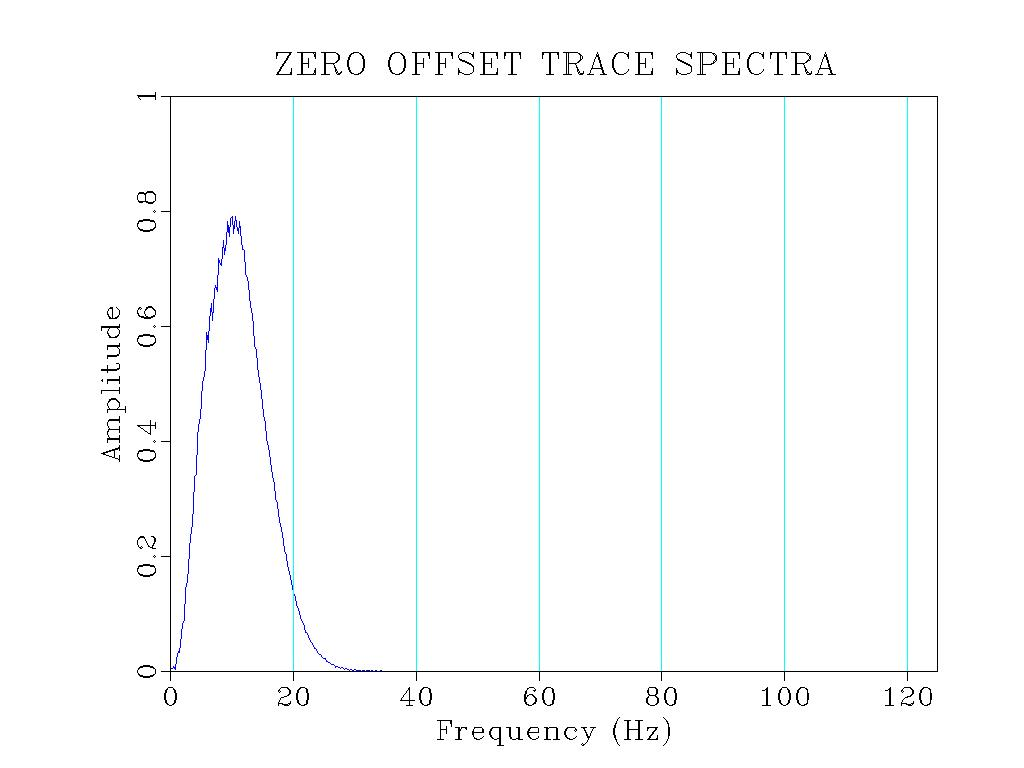
\includegraphics[scale=0.4]{images/originalTraceSpectra.jpeg}
\vspace{-0.3cm}
\end{center}
\begin{center}
 Fonte: Do Autor.
\end{center}
\label{fig:7.1}
\end{figure}


\begin{figure}
\caption{Resultado do empilhamento ERC: Supertraço para m0=4Km. A interpolação e o empilhamento ERC adicionam
ruído numérico aos dados empilhados.}
\begin{center}
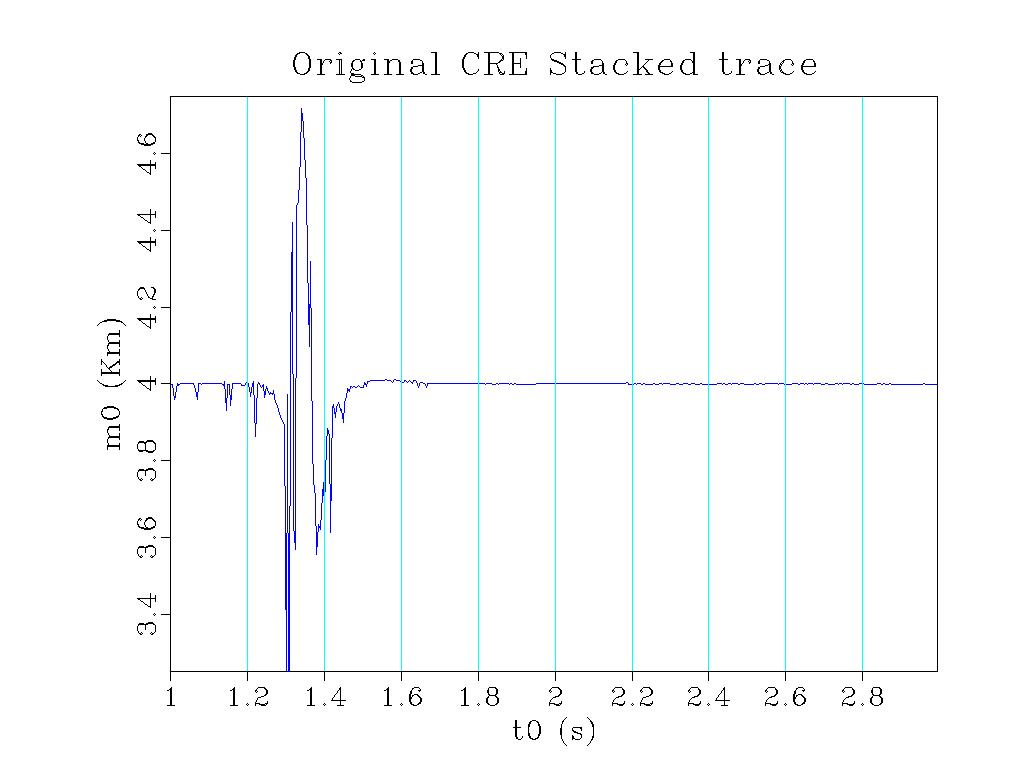
\includegraphics[scale=0.4]{images/creStackedSection.jpeg}
\vspace{-0.3cm}
\end{center}
\begin{center}
 Fonte: Do Autor.
\end{center}
\label{fig:7.2}
\end{figure}

\begin{figure}
\caption{Espectro de amplitude original do supertraço ERC para m0=4Km.}
\begin{center}
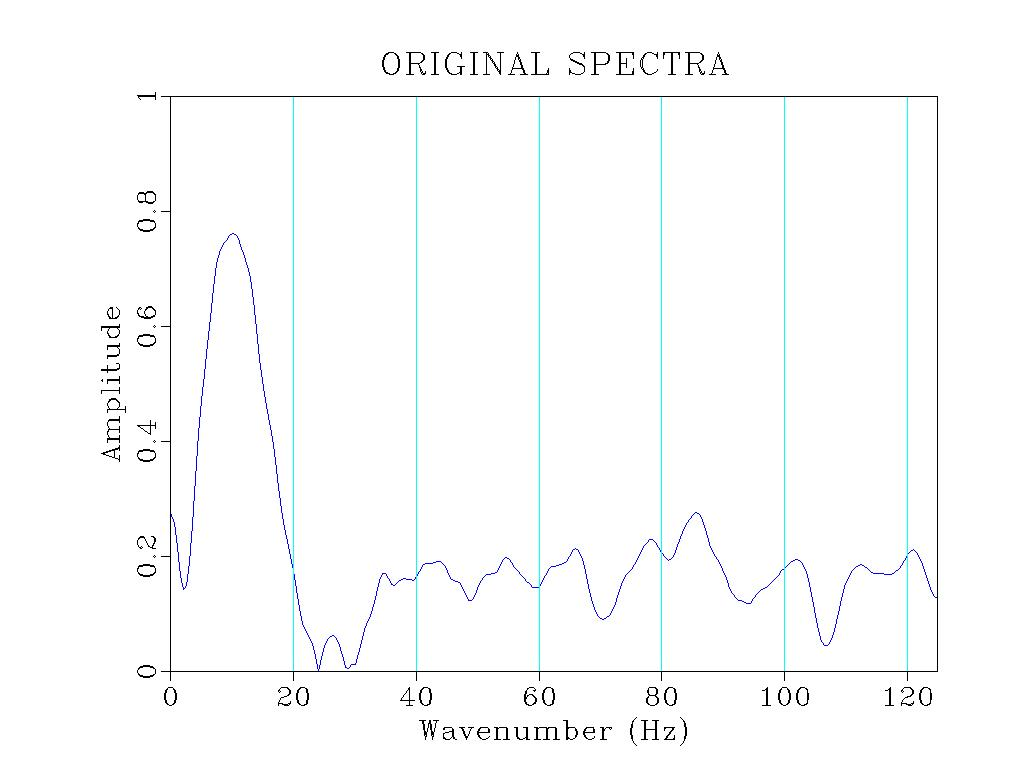
\includegraphics[scale=0.4]{images/originalSpectra.jpeg}
\vspace{-0.3cm}
\end{center}
\begin{center}
 Fonte: Do Autor.
\end{center}
\label{fig:7.3}
\end{figure}

\begin{figure}
\caption{Supertraço cre após a filtragem banda passante.}
\begin{center}
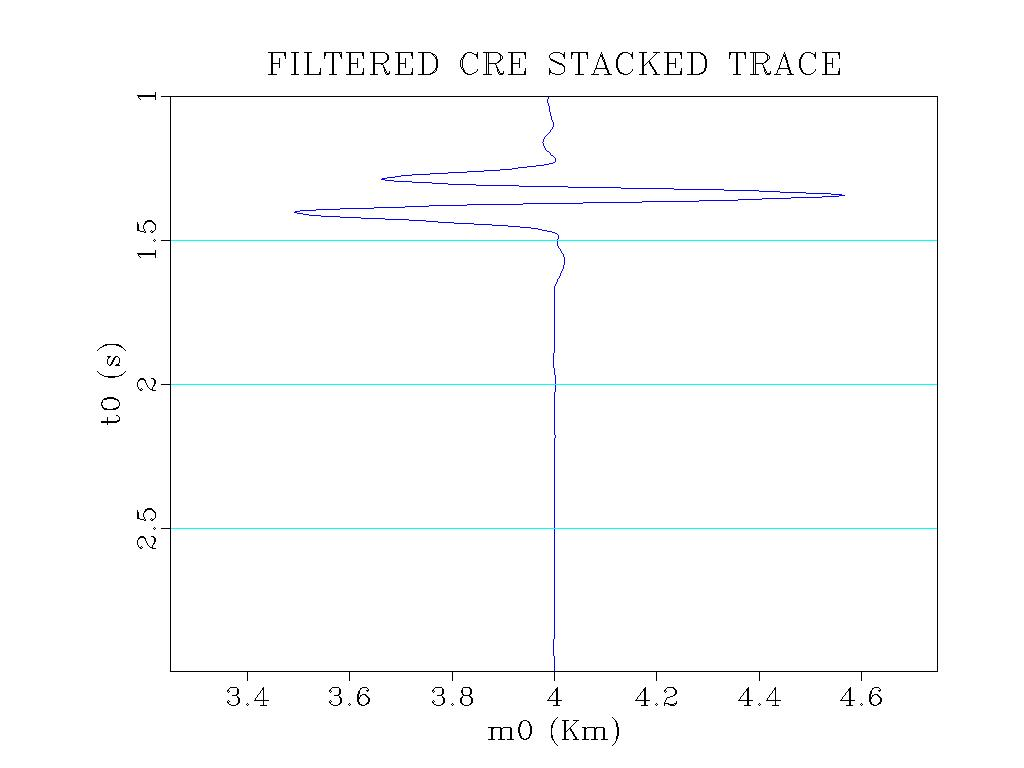
\includegraphics[scale=0.4]{images/creStackedSectionFiltered.jpeg}
\vspace{-0.3cm}
\end{center}
\begin{center}
 Fonte: Do Autor.
\end{center}
\label{fig:7.4}
\end{figure}

\begin{figure}
\caption{Espectro de amplitude após a filtragem banda passante.}
\begin{center}
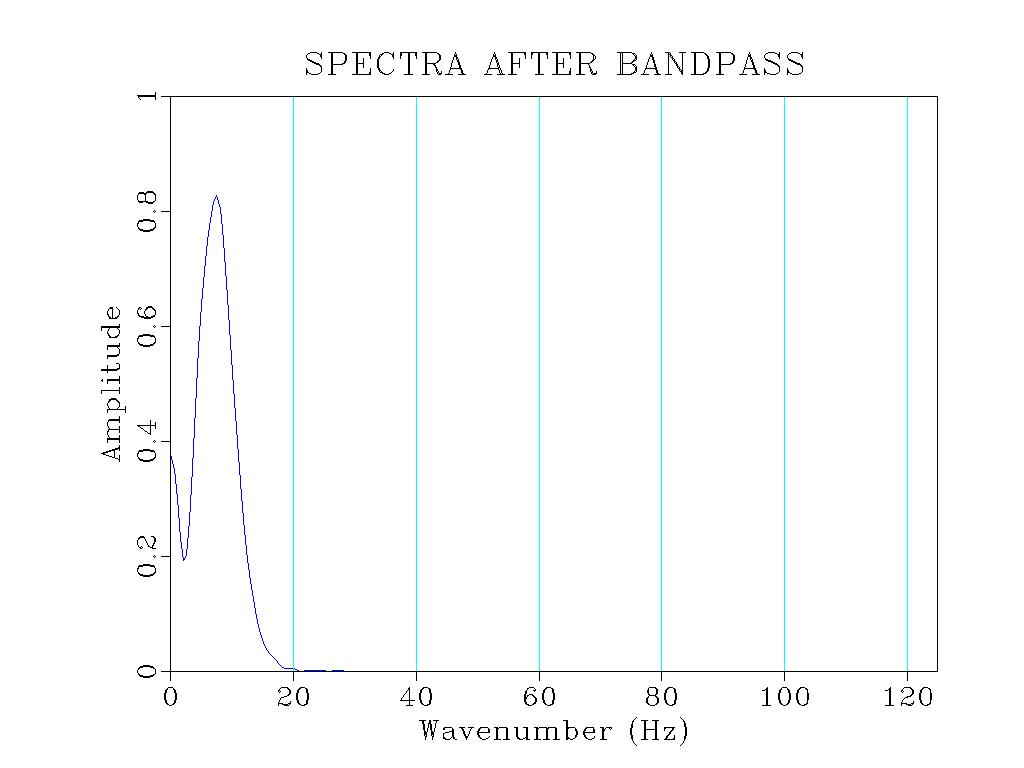
\includegraphics[scale=0.4]{images/filteredSpectra.jpeg}
\vspace{-0.3cm}
\end{center}
\begin{center}
 Fonte: Do Autor.
\end{center}
\label{fig:7.5}
\end{figure}

